\begin{appendices}

  \begin{figure}[H]
  \center
  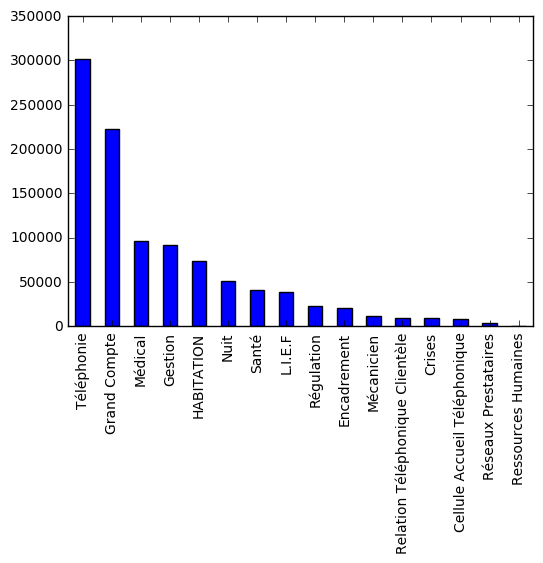
\includegraphics[scale=0.7]{img/description_features.png}
  \caption{Values of the different categories to be predicted}
  \label{des_fig}
  \end{figure}

  \begin{figure}[H]
  \center
  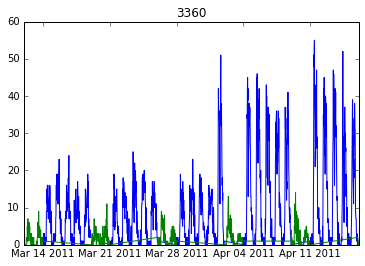
\includegraphics[scale=0.7]{img/holiday.png}
  \caption{Number of calls during worked day (in blue) and holiday (in green)}
  \label{holiday}
  \end{figure}

  \begin{figure}[H]
  \center
  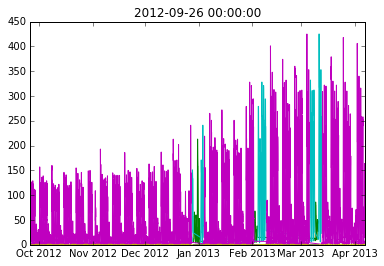
\includegraphics[scale=0.7]{img/res_naive.png}
  \caption{Result in the naive algorithm}
  \label{res_naive}
  \end{figure}

  \begin{lstlisting}[caption=Create the recurrent neural network with 28 outputs, label={RNN}, language=python]
    X = np.concatenate((x_holidays, x, mean_over_time), axis=1)
    _, nb_features = X.shape

    # Model creation
    batch = 336
    main_input = Input(batch_shape=(batch, 1, nb_features), name='main_input')
    lstm = LSTM(32, stateful=True)(main_input)
    drop = Dropout(0.5)(lstm)
    outputs = []
    for i in range(28):
        outputs.append(Dense(1, name='out{0}'.format(i))(drop))
    model = Model(input=main_input, output=outputs)
    model.compile(optimizer='adam', loss='mean_squared_error')
    model.load_weights('../dataChallenge/weights/stateful/model_36624_36959_loss_2.5011280818.h5')
  \end{lstlisting}

  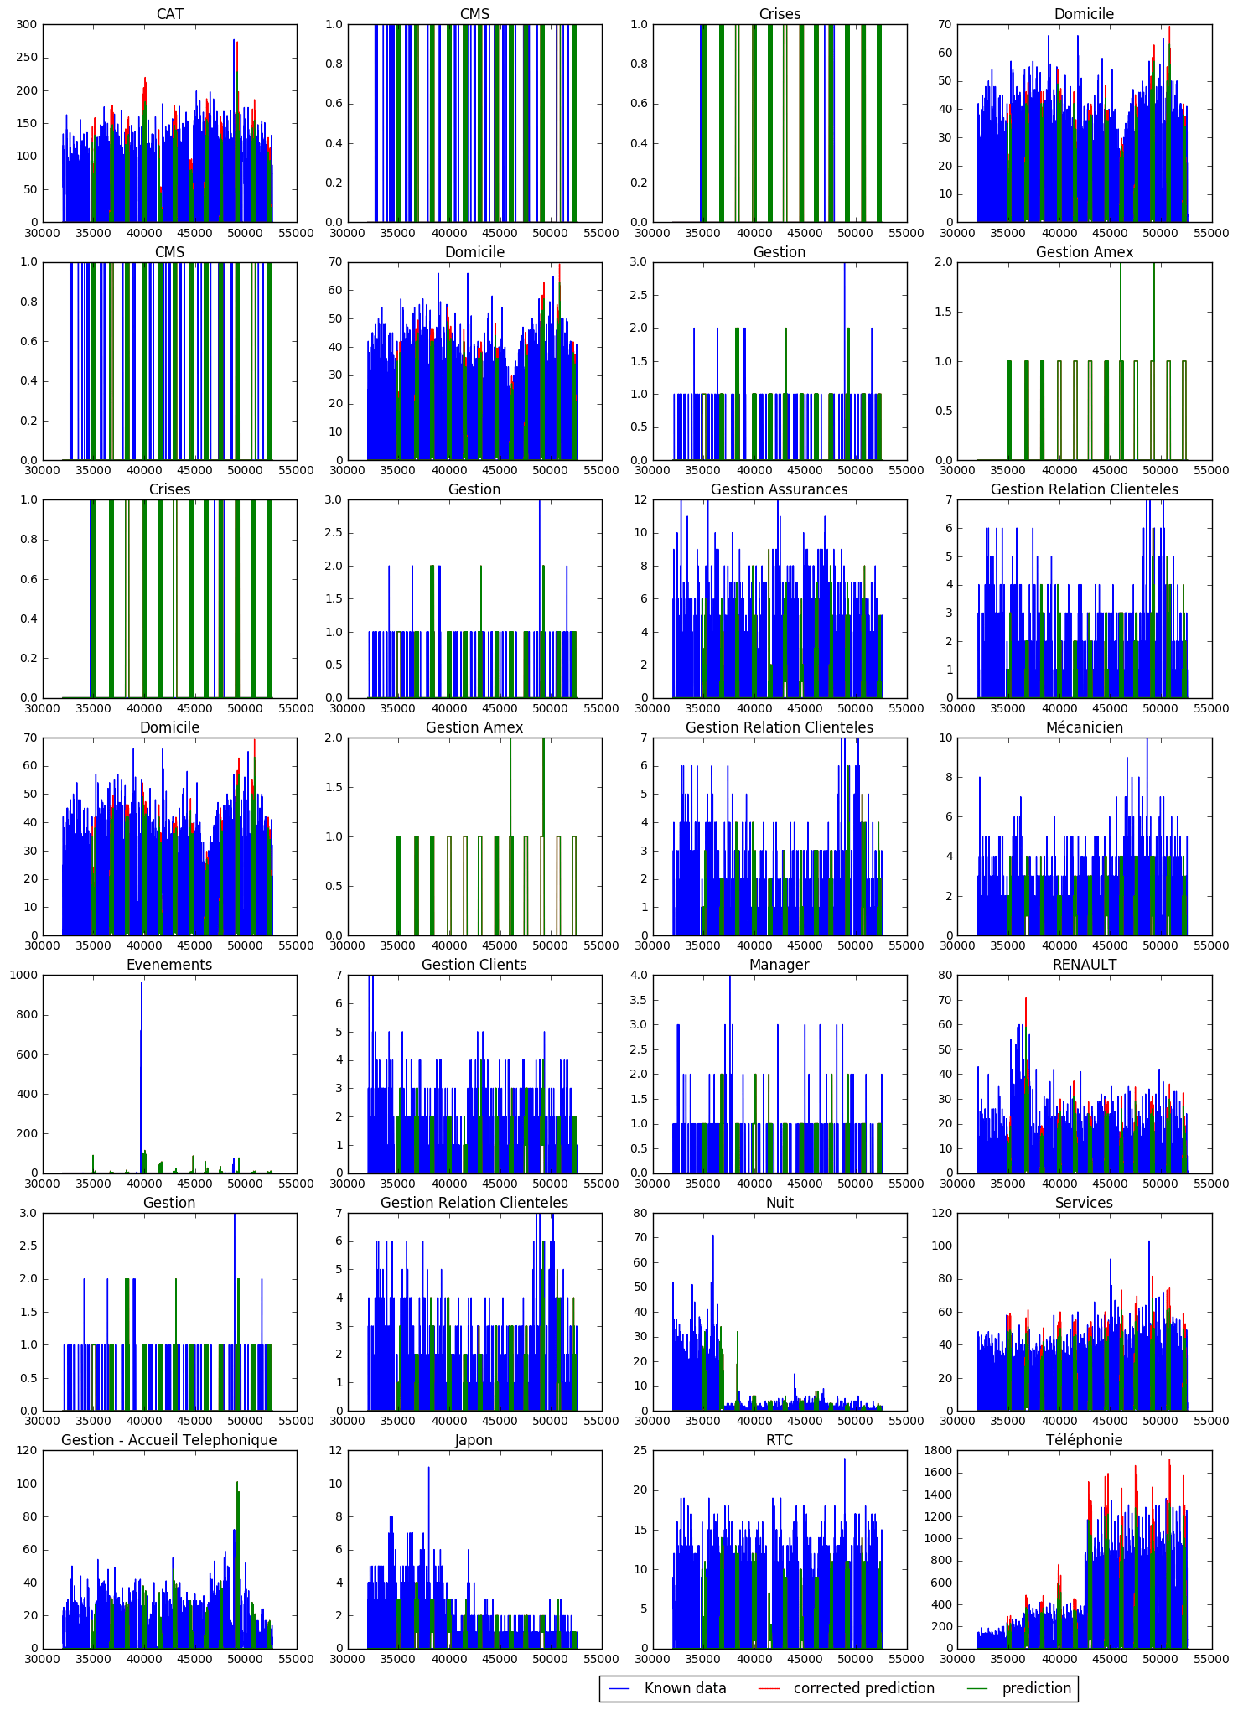
\includepdf{img/plot.pdf}\label{bestmodel}




\end{appendices}
